\documentclass[../document]{subfiles}
\begin{document}
\section{Requirements}
\label{requirements}

\subsection{Sprint 1-3 Requirements}

We are using the goal driven requirement development method to gather our requirements. The first part of this document will be a top down goal level view, with a main goal and sub goals. Then, the second part will give a longer and more detailed textual description for some of the important requirements, followed by a table with a short description for each functional requirement. Finally, the last part of the requirements will present pictures and textual descriptions showing each of the three different views that we will implement.

\subsubsection{Top Goal of the System}
\begin{itemize}
\item
Gather data and present the data visually
\begin{itemize}
\item
Data storage requirement
\begin{itemize}
\item
Write data
\item
Pull data
\end{itemize}
\item
Central hub requirement
\begin{itemize}
\item
Gather data from sensor
\item
Process data
\item
Send data upon request
\end{itemize}
\item
Visualizer requirement
\begin{itemize}
\item
Pull data from the database
\item
Show the data on the GUI
\begin{itemize}
\item
Show a table containing sensors and their data value (temperature, humidity etc)
\item
Show a map with sensors and their position if possible
\item
Map will showcase the temperature, humidity, pressure and lighting near the sensor
\end{itemize}
\item
Allow the user to choose what data to be showcased; the user can choose to turn off temperature, humidity or anything else they please.
\end{itemize}
\end{itemize}
\end{itemize}

\subsubsection{Technological Requirement}
There are certain technologies and methods that we are required to use. These are the result of customer feedback and after a group evaluation and discussion they will be used in the project, if time permits. One of these technology requirements is the database. We are required to use our customers database. This database is supported by our customer and using this would help our customer integrate our project into their format. We are also going to use the same interface classes our customer is using, which is the second technological requirement. Using these interface classes we are able to create an event-driven architecture that closely resembles our customers previous projects, which is what our customer wishes for.

\subsubsection{Database Interaction Requirement}
There will be a database where the data collected from the sensors are stored. The data will include time of recording, sensor identification, location if applicable and measured values such as temperature and lighting. The data can be pulled out later by other modules to be used.

\begin{table}[H]
\caption{Database Interaction Requirements}
\centering
\begin{tabularx}{\textwidth}{|l|L{2.5cm}|X|}
\hline
Req. nr
&Name
&Description
\\ \hline 1.1
&Storing data
&The central hub can push data into the database
\\ \hline 1.2
&Pull data
&The visualizer can pull data out of the database
\\ \hline 
\end{tabularx}
\end{table}

\subsubsection{Central Hub Requirement}
The main task of the central hub is to gather the information and send it to the client when requested, central hub will also process the information to the format we need. The central hub consist of hardware and software. The hardware part is the sensor itself. Because this is provided by the customer, the requirement part is not necessary. The software server will function as a gather, process and send unit, which gathers data from the sensors, process it and forwards the data if requested.

\begin{table}[H]
\caption{Visualizer Requirements}
\centering
\begin{tabularx}{\textwidth}{|l|L{2.5cm}|X|}
\hline
Req. nr
&Name
&Description
\\ \hline 2.1
&Gather data from sensor
&The sensor data will be collected by the server.
\\ \hline 2.2
&Store data
&The central hub will store information it has pooled from the sensors into the database.
\\ \hline 2.3
&Process data 
&The central hub will process data into the form the visualizer needs.
\\ \hline 2.4
&Support hotjoin
&Sensors should be able to disconnect and connect to the central hub at will.
\\ \hline 
\end{tabularx}
\end{table}

\subsubsection{Visualizer Requirement}
The visualizer is the main focus of the project. As a result of that this is also the part with most requirements. The visualizer will first gather the data it needs from the database, then present it on a map featuring the position to each sensor. The map will also show the temperature, humidity, pressure and lighting near the sensor. We will also create multiple types of views. One of them will be the traditional table view with the data name on one side and the number on the other, this view will most be used for testing and verifying data. The other one will show the sensors in a 2D environment, with data animation.

\begin{table}[H]
\caption{Visualizer Requirements}
\centering
\begin{tabularx}{\textwidth}{|l|L{2.5cm}|X|}
\hline
Req. nr
&Name
&Description
\\ \hline 4.1
&Pull data from the database
&The visualizer will be able to pull data from the database in regular intervals.
\\ \hline 4.2
&Show the data on the GUI
&The data will be displayed in a window.
\\ \hline 4.2.1
&Present data in a table
&The data collected will be placed in a table with the data type on the right, and the value on the left.
\\ \hline 4.2.2
&Present data in a map with sensors
&We will construct a map containing sensors and possibly their position. The data, such as temperature, will be displayed near each sensor.
\\ \hline 4.2.3
&Adding a system clock
&A clock to track time for all activities on the system.
\\ \hline 4.3
&Allow user to switch between different data type
&The user should be able to select what kind of data type they want to see in order to not confuse himself with so much data on the screen.
\\ \hline 
\end{tabularx}
\end{table}

\newpage

\subsubsection{Table View}
This is the view where all sensors and the data is showcased in a table. The sensor number can be seen on the left and the data from the sensors can be seen in the appropriate row. If the user prefers less information he can click on the checkbox on the right to hide information that is unwanted.

\begin{figure}[H]
\centering
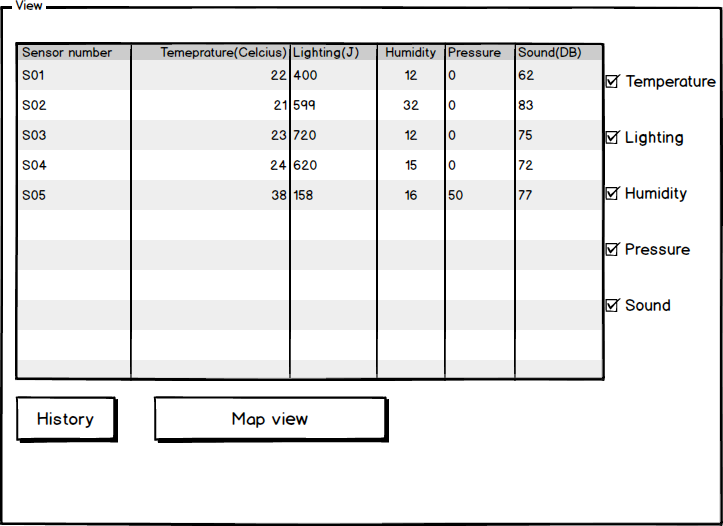
\includegraphics[width=\textwidth]{requirements/table_view.png}
\caption{Table View}
\end{figure}

\newpage

\subsubsection{Map View}
The map view will make an illustration of the room. In the real model the data will be shown in the form of image manipulation, not a function in the mockup program. If position can be tracked we will do so, otherwise we must find another way to show the data in a 2D map.

\begin{figure}[H]
\centering
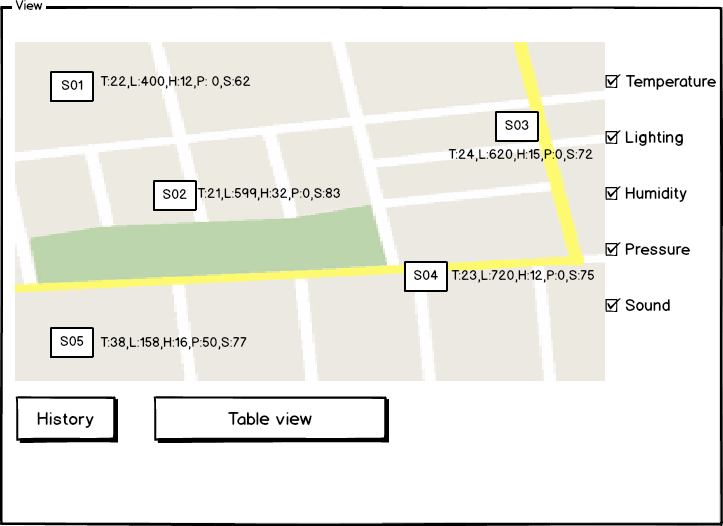
\includegraphics[width=\textwidth]{requirements/map_view.png}
\caption{Map View}
\end{figure}

\subsection{Sprint 4 Requirements}

After finishing sprint 3 and reviewing the final prototype with the customer, he had some input on things that we should change. Although we did not have much time we left, we took the challenge and added new requirements to our program. The requirements were mostly concerned with visualisation of multiple gateways and the use of link budget to visualise sensor position. For each sensor and gateway pair we have a link budget. The link budget works like a ping system. It accounts for losses and gains of radio signals through a medium, and reports that in a unit of value. We have found out that the link budget varies in between forty and one hundred. The higher the link budget, the theoretically larger the distance between it and the central hub. By having multiple gateways, at least three, we are able to trilaterate the position of the sensor in the visualiser.

Below we will represent these new requirements, first as a top-down representation, and then as a table.

\begin{itemize}
	\item
	Visualise multiple gateways and positions of each sensor using link budget
	\begin{itemize}
		\item
		Visualiser supports multiple gateways
		\begin{itemize}
			\item
			Drawing of the gateway on the visualiser, by using a geometric pattern
		\end{itemize}
		\item
		Implementing link budget variable
		\begin{itemize}
			\item
			One link budget for each gateway sensor pair
			\item
			Using link budgets as weights to calculate the position of the sensor
			\item
			Sensors will be able to move during runtime if link budget changes
			\item
			If the sensor moves too far away the visualiser will reflect that
			\item
			The administrator can configure a file containing scaling for link budget
		\end{itemize}
		\item
		Make a random data generator for testing and simulation purposes
		\begin{itemize}
			\item
			The random data generator should generate data in the pattern that is similar to real life instances
		\end{itemize}
	\end{itemize}
\end{itemize}
	
\begin{table}[H]
\caption{Description}
\centering
\begin{tabularx}{\textwidth}{|l|L{2.5cm}|X|}
\hline
Req. nr
&Name
&Description
\\ \hline 5.1
&Multiple gateways
&The visualiser will support multiple gateways. The total number of gateways will be adjustable freely, and depends on the data. This means we can add as many gateways as we want.
\\ \hline 5.1.1
&Gateway positioning
&These gateways will be positioned in a geometric pattern showcasing how they would be placed in a perfect set up. 
\\ \hline 5.2
&Link budget
&The sensors have a value called the link budget. The link budget extends our models.
\\ \hline 5.2.1
&Position calculation
&We will use the link budgets as weights to calculate the position of the sensor.
\\ \hline 5.2.2
&Implementing link budget
&Each gateway and sensor pair have one link budget each, unless the sensor goes out of the range.
\\ \hline 5.2.3
&Animation of position
&The sensors will be able to move freely during runtime if the link budget changes
\\ \hline 5.2.4
&Out of range animation
&If the sensor moves too far away from a gateway the signal should reflect that.
\\ \hline 5.2.5
&Link budget calibration
&The administrator can configure a .txt file containing scaling for link budget, meaning how large the link budget needs to be before we consider the link budget as out of range.
\\ \hline 5.3
&Random data generator
&Make random data generator for the database
\\ \hline 5.3.1
&Generate data
&The random data generator should generate data in the pattern that is similar to real life instances
\\ \hline 
\end{tabularx}
\end{table}
















\end{document}